\section{Aufbau Bot}
\label{sec:module.AufbauBot}

Dieses Kapitel beschreibt die Klassenhierarchie unserer Bot Implementation.

\subsection{Klasse Bot}
\label{sec:module.Bot.Bot}

\begin{figure}[H]
\centering
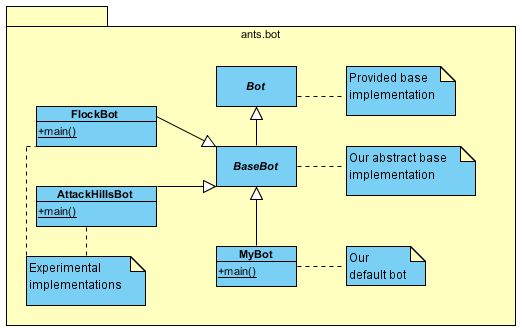
\includegraphics[width=0.7\textwidth]{91_bilder/antsBot}
\caption[Bot Klassenhierarchie]{Vererbung der Bots wobei auf Stufe impl (Implementation) nur MyBot verwendet wird.}
\label{fig:antsBot}
\end{figure}

Als Basis f�r unsere Bot Implementation haben wir den Beispiel-Bot (Klasse Bot.java) verwendet, der im Java-Starter-Package enthalten ist. Das Starter-Package kann von der AI-Challenge Website\footnote{http://aichallenge.org/ants\_tutorial.php} heruntergeladen werden. Der Bot erweitert die Klassen AbstractSystemInputReader und AbstractSystemInputParser, welche die Interaktion mit der Spielengine �ber die System-Input/Output Streams kapseln. F�r eine optimierte L�sung k�nnte der Bot auch angepasst werden, indem er selber auf die Streams zugreift. Im Rahmen dieser Arbeit erschien uns das nicht n�tig. Die Klasse Bot dient als Grundlage f�r die Klasse BaseBot, welcher wiederum Grundlage ist f�r die Klasse MyBot, wie Abb. \ref{fig:antsBot} illustriert.
Die Klasse BaseBot wurde in erster Linie eingef�hrt, um m�glichst einfach verschiedene Bot Implementierungen zu Testzwecken schreiben zu k�nnen (s. Kapitel \ref{sec:testCenter.Testbots}).

Die Bot Implementierungen verf�gen jeweils �ber die Einsprungs-Methode \texttt{main()}, die im einfachsten Fall aus einer einzelnen Zeile besteht (z.B. \texttt{new FlockBot().readSystemInput();}). Listing \ref{lst:mainMethod} zeigt die \texttt{main()}-Methode von MyBot.

\lstset{language=Java, tabsize=4}
\begin{lstlisting}[caption=Main-Methode von MyBot, label=lst:mainMethod]
public static void main(String[] args) throws IOException {
        // we only support one arg, and that is assumed to be the profile name
        String profile = args.length == 1 ? args[0] : null;
        initLogging(profile);
        new MyBot(profile).readSystemInput();
    }
		
\end{lstlisting}

\subsection{BaseBot}
\label{sec:module.Bot.BaseBot}

Die abstrakte Klasse BaseBot erbt von Bot. Hier haben wir die Struktur unseres Spielzuges definiert.

\subsection{Ablauf eines Zugs} 
\label{sec:implementation.Bot.Turn}

\begin{figure}[H]
\centering
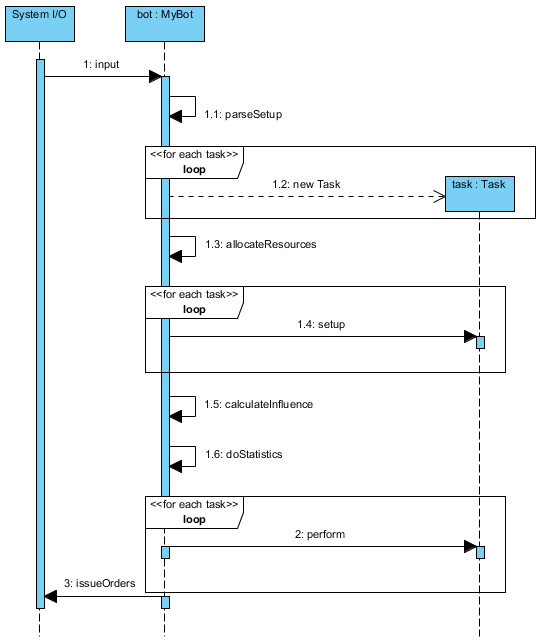
\includegraphics[width=0.9\textwidth]{91_bilder/FirstTurn}
\caption{Ablauf des ersten Zugs des Spiels}
\label{fig:firstTurn}
\end{figure}

Abbildung \ref{fig:firstTurn} zeigt den Ablauf des ersten Zugs, w�hrend Abbildung \ref{fig:turn} den Ablauf aller weiteren Z�ge zeigt. 

\begin{figure}[H]
\centering
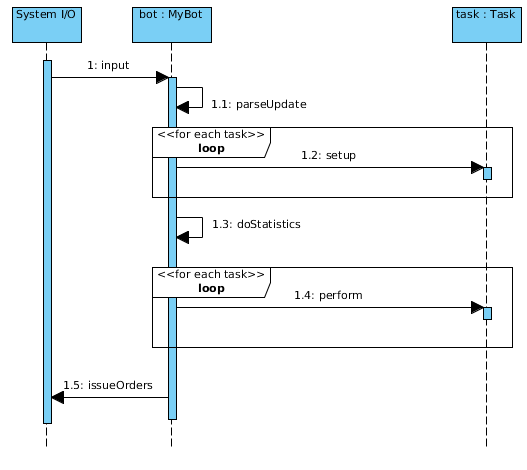
\includegraphics[width=0.9\textwidth]{91_bilder/Turn}
\caption{Ablauf der weiteren Z�ge des Spiels}
\label{fig:turn}
\end{figure}

Jeder Zug beginnt mit dem Einlesen des Inputs vom SystemInputStream. Wenn der Bot das Signal ''READY`` (1. Zug) oder ''GO`` (alle weiteren Z�ge) erh�lt, kann er den gesammelten Input verarbeiten (Methode \texttt{parseSetup()} respektiv \texttt{parseUpdate()}). Danach wird die eigentliche Logik des Bots in der Methode \texttt{doTurn(...)} ausgef�hrt.

Im 1. Zug werden dabei Instanzen der Tasks erstellt. Abgesehen davon unterscheidet sich der 1. Zug von diesem Punkt an nicht mehr von allen nachfolgenden Z�gen. Die Tasks werden vorbereitet (Aufruf der jeweiligen \texttt{setup()} Methode. Danach werden einige statistische Werte aktualisiert und in jedem 10. Zug auch geloggt. Dann werden die Tasks in der definierten Reihenfolge aufgerufen. Hier wird der L�wenanteil der Zeit verbracht, denn die Tasks enthalten die eigentliche Logik unserer Ameisen.

Zum Schluss werden dann mit \texttt{issueOrders()} die Z�ge der Ameisen �ber den SystemOutputStream an die Spielengine �bergeben. Im Code sieht das ganze folgendermassen aus.

\lstset{language=Java, tabsize=4}
\begin{lstlisting}[caption=Der Ablauf des Spielzuges, label=lst:ablaufspielzug]
@Override
/*
 * This is the main loop of the bot. All the actual work is
 * done in the tasks that are executed in the order they are defined.
 */
public void doTurn() {
		// write current turn number, ants amount into the log file.
	addTurnSummaryToLogfiles();
		// new calculation of the influence map
	calculateInfluence();
		// write some statistics about our population
	doStatistics();
		// initialize the task (abstract method) must be implemented by the inherited class
	initTasks();
		// execute all task (main work to do here)
	executeTask();
		// write all orders to the output stream
	Ants.getOrders().issueOrders();
		// log all ants which didn't get a job.
	logUnemployedAnts();
}
\end{lstlisting}


\subsection{MyBot}
\label{sec:module.Bot.MyBot}

Wie bereits im Listing \ref{lst:ablaufspielzug} ersichtlich, ist die Methode \texttt{initTasks()} in BaseBot abstrakt und muss von MyBot implementiert werden. \texttt{initTasks()} definiert welche Tasks, oder besser gesagt F�higkeiten der Bot hat. Dies wurde ausgelagert, da nicht nur MyBot von BaseBot erbt, sondern auch weiter Bots die wir zu Testzwecken erstellt haben um nur gewisse Funktionalit�ten zu testen. (Siehe dazu \ref{sec:testCenter.Testbots}) Weiter wird in der \texttt{main()}-Methode von MyBot \texttt{initLogging(...)} aufgerufen. Hier definieren wir, welche Logkategorien mit welchem Loglevel ins Logfile geschrieben werden. (Mehr zum Thema Logging siehe Kapitel \ref{sec:module.Logging}). Je nach Modul, das gerade getestet wird kann die Anzahl Logeintr�ge justiert werden.\\
MyBot initialisiert die folgend aufgef�hrten Tasks; es sind die Tasks, die sich im Lauf der Arbeit bew�hrt haben. Die detaillierte Beschreibung der Tasks ist im nachfolgenden Kapitel \ref{sec:module.Tasks} zu finden.

\begin{itemize}
		\item GatherFoodTask
		\item AttackHillsTask
		\item DefendHillTask
		\item ExploreTask
		\item ClearHillTask
		\item CombatTask
		\item ClusteringTask
\end{itemize}